\documentclass[11,aspectratio=1610]{beamer}
\usepackage[utf8]{inputenc}
\usepackage{mathrsfs}  
\usepackage{xcolor}
\usepackage{setspace}
\usepackage{comment}
\usepackage{hyperref}
% config du thgeme metropolis
\usetheme[progressbar=frametitle,block=fill, titleformat=smallcaps,sectionpage=progressbar,]{metropolis}



\title{Resilience and stability of ecological systems}
\subtitle{an awesome paper by C.S. Holling}
\date{}
\author{}



\definecolor{links}{HTML}{60bbf7}
\hypersetup{colorlinks,linkcolor=,urlcolor=links}


%definition de la couleur du texte dans la balise \alert{}
\definecolor{vertIGN}{HTML}{96C31E} % vert IGN %vrai valeur #97BE0D
\setbeamercolor{alerted text}{fg=vertIGN}

\definecolor{grisIGN}{HTML}{22292F} % Gris IGN tiré vers le noir 
\setbeamercolor{background canvas}{bg=grisIGN}




% code pour placer le log ENSG dans le bandeau des slides titre 
\makeatletter
\setbeamertemplate{frametitle}{%
  \nointerlineskip%
  \begin{beamercolorbox}[%
      wd=\paperwidth,%
      sep=0pt,%
      leftskip=\metropolis@frametitle@padding,%
      rightskip=\metropolis@frametitle@padding,%
    ]{frametitle}%
  \metropolis@frametitlestrut@start%
  \insertframetitle%
  \nolinebreak%
  \metropolis@frametitlestrut@end%
  \hfill
  \raisebox{-0.6ex}{
\includegraphics[height=2.5ex,keepaspectratio]{img/logo_LASTIG.png}}
  \end{beamercolorbox}%
}
\makeatother




% logo ENSG première page 
\titlegraphic{\flushright
\includegraphics[height=1cm]{img/logo_LASTIG.png}

\vspace{7cm}
\centering

%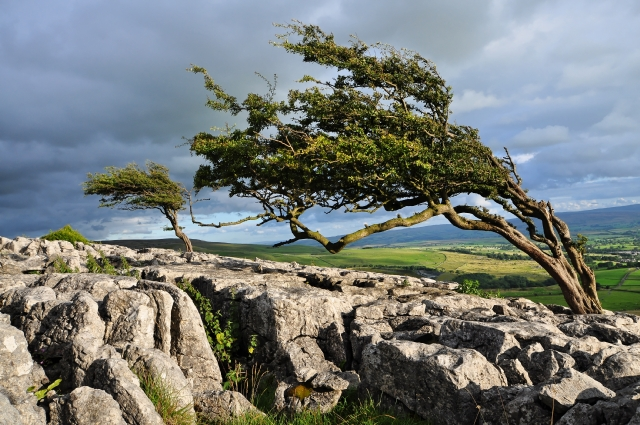
\includegraphics[height=4cm]{img/resilient_tree.jpg}\\

\begin{scriptsize}LASTIG Reading Group - summer 2024 - paul \end{scriptsize}
} 



\begin{document}
\metroset{background=dark} % change background theme according to manual
\maketitle  




\begin{frame}{Disclaimer}

This talk contains 
\begin{itemize}
  \item no AI
  \item no GIS
  \item no maps
  \item no LASTIG specific topic
  \item no expertise
\end{itemize}

\end{frame}


\section{The Author} 

\begin{frame}{C.S. Holling, the man, the legend}



 \begin{columns}
          \column{0.38\textwidth}
             \centering
             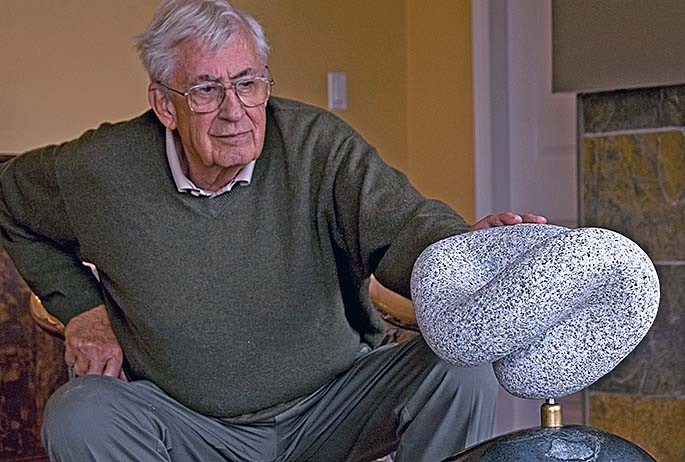
\includegraphics[width=\textwidth]{img/Holling.jpg}
           \column{0.58\linewidth}
\begin{scriptsize}
Crawford Stanley "Buzz" Holling, (1930 - 2019)

\begin{itemize}
  \item PhD in 1957
  \item worked several years in the Canadian Forestry Departement 
  \item Professor and Director of the Institute of Animal Resource Ecology, Univ. of British Columbia 
  \item Awarded multiple times
\end{itemize}
\end{scriptsize}
\end{columns}

\begin{small}
\vspace{1cm}
Father of the concept of \alert{resilience}, adaptive management, adaptive cycle, and panarchy. 

\vspace{0.5 cm}
Pionneer in interdsciplinary and participatory \alert{modeling workshops} about \alert{natural systems management}. 




\end{small}

\end{frame}


\section{Ecological modeling in three slides}




\begin{frame}{(1) Silver Springs model  }
Energy flows in a natural system [Odum,  1971]
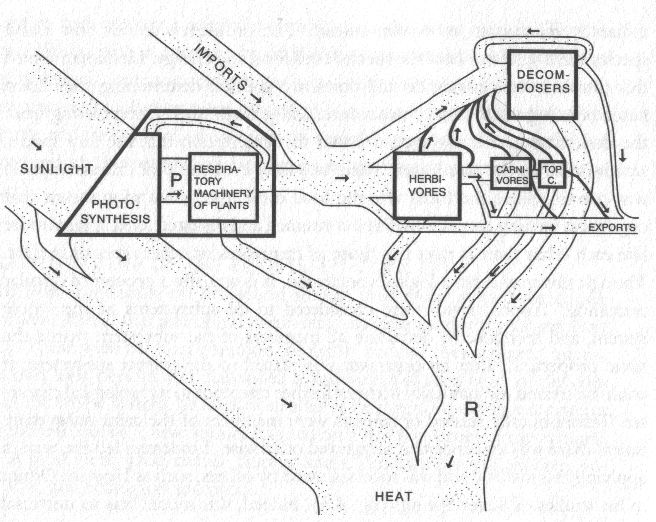
\includegraphics[width=0.8\textwidth]{img/Silver_Spring_Model.jpeg} 

\tiny{image  : via wikipedia from:  Odum, H.T. (1971). Environment, Power, and Society. Wiley-Interscience New York, N.Y.}
\end{frame}



\begin{frame}{(2) Functional responses}
\begin{scriptsize}

 \begin{columns}
          \column{0.38\textwidth}
             \centering
             \colorbox{white}{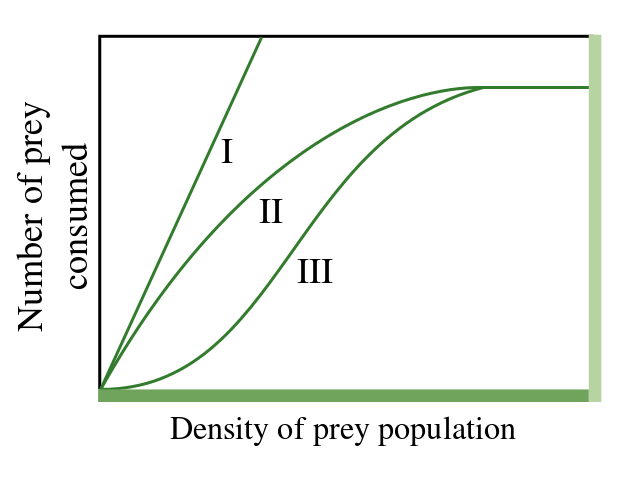
\includegraphics[width=\textwidth]{img/FunctionalResponses.png}}
           \column{0.58\linewidth}

\begin{itemize}
  \item early work of Holling ~ 
  \item Model the relationships between preys density and consumption 
  \item Type I models instant consumption (no chase, no boundaries) 
  \item Type II models saturation for high prey densities (short chase, early satitation )
  \item Type III models a learning phase in chasing preys  and selection of preys (rare)
\end{itemize}
\end{columns}

\vspace{1cm}

$\rightarrow$ real predators feed on several preys, combining Type II and Type III 
\end{scriptsize}
\end{frame}


\begin{frame}{(3) Ecosystem modeling }


\begin{columns}
          \column{0.7\textwidth}
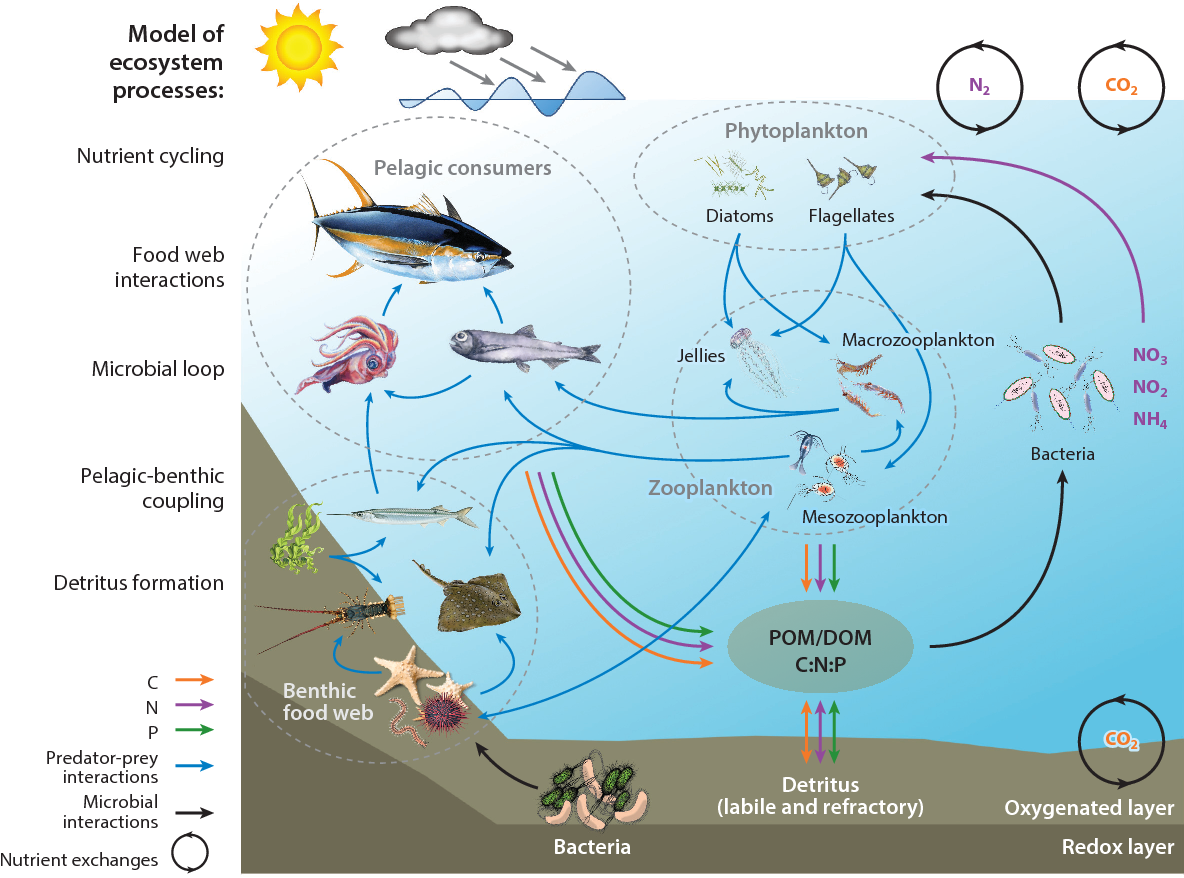
\includegraphics[width=0.9\textwidth]{img/ecosystem_model.png}
\column{0.4\textwidth}
\scriptsize{
An \alert{ecosystem model} represent the system formed by a bunch of species interacting with and within an environment


\vspace{0.5cm}
  \alert{Each arrow}  has to be modelled  e.g. Functional responses  model the evolution of thuna pop. regarding its preys
}
\end{columns}



\vfill
\tiny{Image from :  Pethybridge, Heidi R. et al. “Improving Marine Ecosystem Models with Biochemical Tracers.” Annual review of marine science 10 (2018): 199-228.}

\end{frame}





\section{The Paper}

\begin{frame}[standout]

\begin{quote}
"Individuals die, population disappear and species become extinct. That is one view of the world."
\end{quote}
\flushright
\tiny{(the first two lines of the paper)}
  
\end{frame}




\begin{frame}{Two perspectives on system}

Holling distinguishes two perspectives : 

\vspace{1cm}

\begin{scriptsize}
\begin{columns}
          \begin{column}{0.5\textwidth}
\begin{itemize}
\item when a system is designed to perform a specific task \alert{under a narrow range of predictable external conditions}
\item \alert{consistant non-variable performance} and the amplitude and frequency of oscillations (if any) are important
\item \alert{Quantitative} view is preferred : how much more ? how long ? 
\end{itemize}      
\end{column}
\vrule
\begin{column}{0.5\textwidth}
\begin{itemize}
\item when a system is profoundly affected by external changes  (i.e.  sensitive)
\item when confronted to \alert{unexpected variations} consistancy of behavior $<<$ \alert{persistence of properties, relationships}
\item \alert{Qualitative} view is preferred : does it exist?  would it disappear  or come back ?
\end{itemize}
\end{column}
\end{columns}
\end{scriptsize}

\end{frame}




\begin{frame}{Quantitative Tradition}


Tradition of analysis is \alert{quantitative} : e.g. physics 

  \vfill

\begin{itemize}
  \item  Equilibrium centered view are static  
  \item  Transient behaviors  (far from equilibrium) are unknown
  \end{itemize}
  \vfill
  Some limitations : 
  \begin{itemize}
  \item  Species populations in equilibrium states won't inform on conditions of persistence 
  \item  Human exploitation shifts natural systems away from their equilibrium
\end{itemize}
\end{frame}
  
  

\begin{frame}{Purpose of the article  : }
Holling delivers \alert{a review of ecological theory} mixed with  {real natural system behaviors} \\ 

\vfill

$\implies$ Would different perspectives yield different useful insights?  

\vfill
Natural systems are \alert{dynamic}, subject to \alert{perturbations} (often human). \\

\vfill
\alert{Persistance, resistance, adaption} are properties of interest






\end{frame}
  

\section{Predators and preys}


\begin{frame}{Lotka Volterra equations}


Theoretical (simple) model of two populations : 

$\color{cyan}{x(t)}$ are preys , $\color{orange}{y(t)}$ are predators  (population over time)


\[
\left\{
 \begin{array}{ccc}  
 \frac{\mathrm{d}\textcolor{cyan}{x(t)}}{\mathrm{d}t}&=&  \alpha \textcolor{cyan}{x(t)} - \beta \textcolor{cyan}{x(t)}\textcolor{orange}{y(t)}\\
 \\
\frac{\mathrm{d}\textcolor{orange}{y(t)}}{\mathrm{d}t}&=&  \delta \textcolor{cyan}{x(t)}\textcolor{orange}{y(t)} - \gamma \textcolor{orange}{y(t)}  \end{array}
\right.
\]

  %  {\displaystyle \left\{{\begin{array}{ccc}{\dfrac {\mathrm {d} x}{\mathrm {d} t}}(t)&=&x(t)\ {\Big (}\alpha -\beta y(t){\Big )}\\{\dfrac {\mathrm {d} y}{\mathrm {d} t}}(t)&=&y(t)\ {\Big (}\delta x(t)-\gamma {\Big )}\end{array}}\right.}

with : 
\begin{footnotesize}
\begin{itemize}
  \item  $\alpha >0$ is prey intrinsic growth rate
  \item  $\beta >0 $ is  prey death  (by predation) rate
  \item  $\gamma >0 $ is predator intrinsic death rate
  \item  $\delta > 0$  is predator growth (by eating preys) rate
\end{itemize}
\end{footnotesize}
\end{frame}


\begin{frame}{Oscillations and stability}


\alert{Patterns} of this system  : 

\begin{itemize}
  \item regulated interactions may lead to \alert{oscillations}
  \item some conditions lead to \alert{extinction}
  \item system may recover from perturbations :  \alert{damping}
\end{itemize}

  
\end{frame}





\begin{frame}{Netlogo demo}

Wolves, sheeps, and grass\\
\vfill
\centering
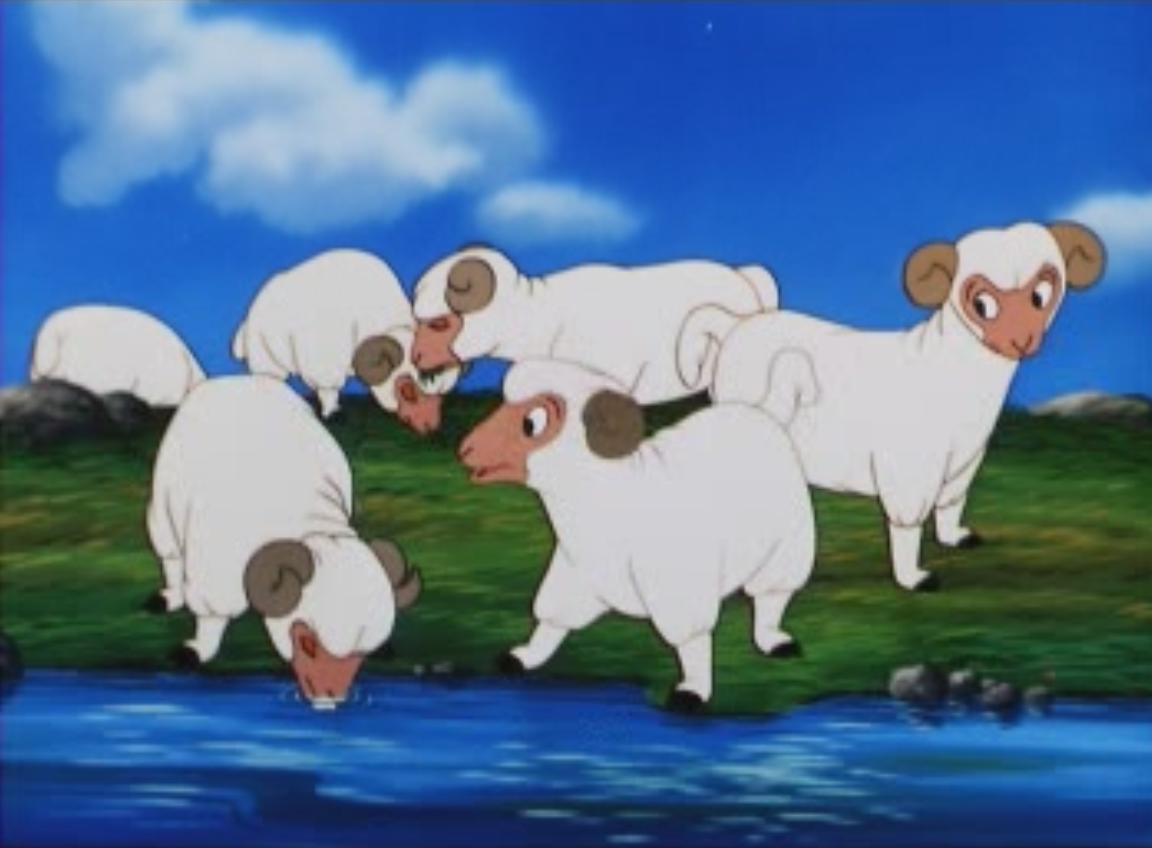
\includegraphics[width=0.45\textwidth]{img/sheep.jpg}

\includegraphics[width=0.45\textwidth]{img/wolf.jpg}\\
\tiny{Lambert the Sheepish Lion, dir. by Jack Hannah © Disney , 1952}
\end{frame}






\begin{frame}{Phase diagram patterns typology}


\centering
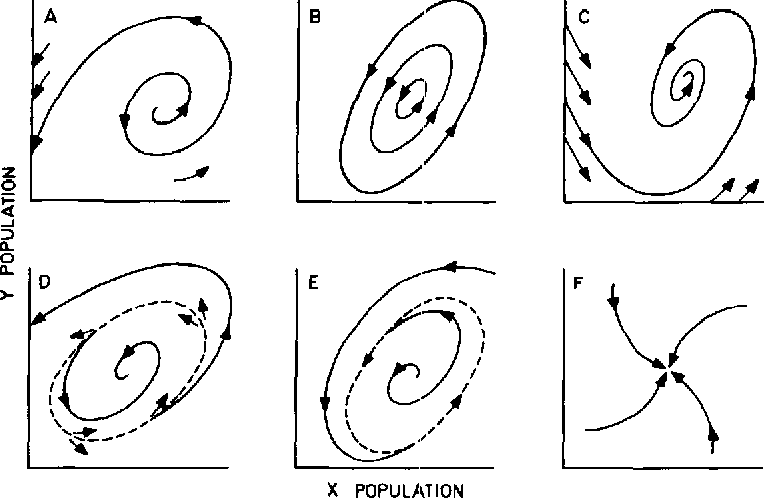
\includegraphics[width=0.5\textwidth]{img/behavior_patterns.png}\\
\flushleft



\scriptsize{A is unstable equilibrium, \\ B is neutrally stable cycles,\\ C is stable equilibrium,\\ D is \alert{domain of attraction},\\ E is \alert{stable limit cycle},\\ F is stable node }

\tiny{obtained by math. analysis. Roughly :  solve derivatives = 0  then apply solutions to the Jacobian matrix, extract the eigen values, real parts signs give (un)stability }


  
\end{frame}


\begin{frame}{"Common" knowledge on these models}

\begin{itemize}
\item all these models have either a stable point  or a stable limit circle (Kolmogorov theorem)
\item a model (given ${\alpha, \beta, \gamma,\delta}$) is either globally stable or globally unstable
\item neutral stability is very unlikely ($\approx$ not attracted by anything) 
\item when stable, a limit cycle is likely  
\end{itemize}

\end{frame}




\begin{frame}{Model Complexification}



\begin{footnotesize}

 \begin{columns}
          \column{0.48\textwidth}
             Relax simplifying assumptions :

\vspace{0.2cm}
\begin{itemize}
  \item several species
\item  add lag in reproduction 
\item  plateau in predators reproduction
\item  non-random predator attacks 
\item  minimum prey density for reproduction 
\end{itemize}

           \column{0.55\linewidth}

$\implies$ D-type patterns \\
\vspace{1cm}
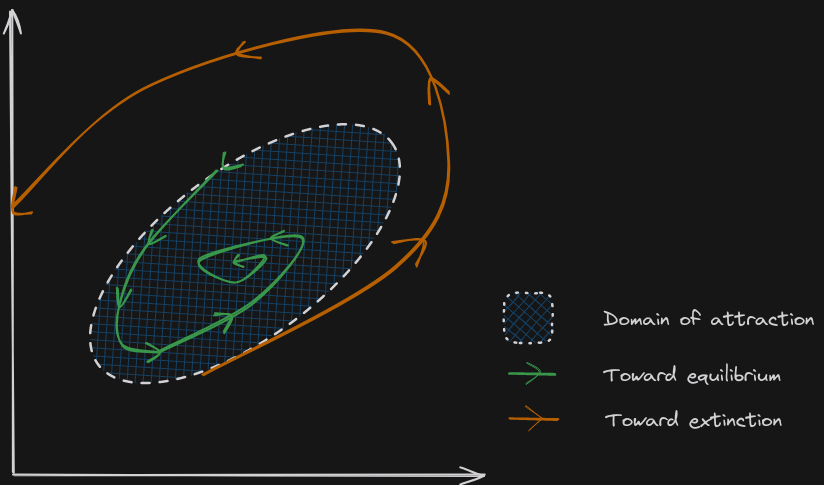
\includegraphics[width=\textwidth]{img/type2D.png}
\vfill
\end{columns}

\end{footnotesize}

\end{frame}



\begin{frame}{Domains of attraction}


More realistic models have : 



\begin{itemize}
  \item  \alert{several distinct} domains of attraction 
  \item stable nodes,
  \item stable limit cycles
\end{itemize}


\vfill



\alert{Size} and \alert{location} of domains  $\leftrightarrow$ \alert{persistence} of the system and \alert{probability of extinction} of  species\\


\vfill


\tiny{Some viability theory should be useful here}


  
\end{frame}




\begin{frame}{Netlogo demo}
\vfill
The Rabbits, Grass, Weeds model in netlogo 
\vfill
\centering

\includegraphics[width=0.6\textwidth]{img/bunny.jpg}

\tiny{Big Buck Bunny, The Blender Fondation, 2008}

  
\end{frame}

\begin{frame}{What differs from equations ? }

Netlogo ABM additions :

\begin{itemize}
  \item discrete populations \& space
  \item three "species"
  \item randomness
  \item spatiality / movement 
\end{itemize}


\end{frame}




\section{Real world closed systems}



\begin{frame}{A lake}
\begin{footnotesize}
 \begin{columns}
           \column{0.48\textwidth}
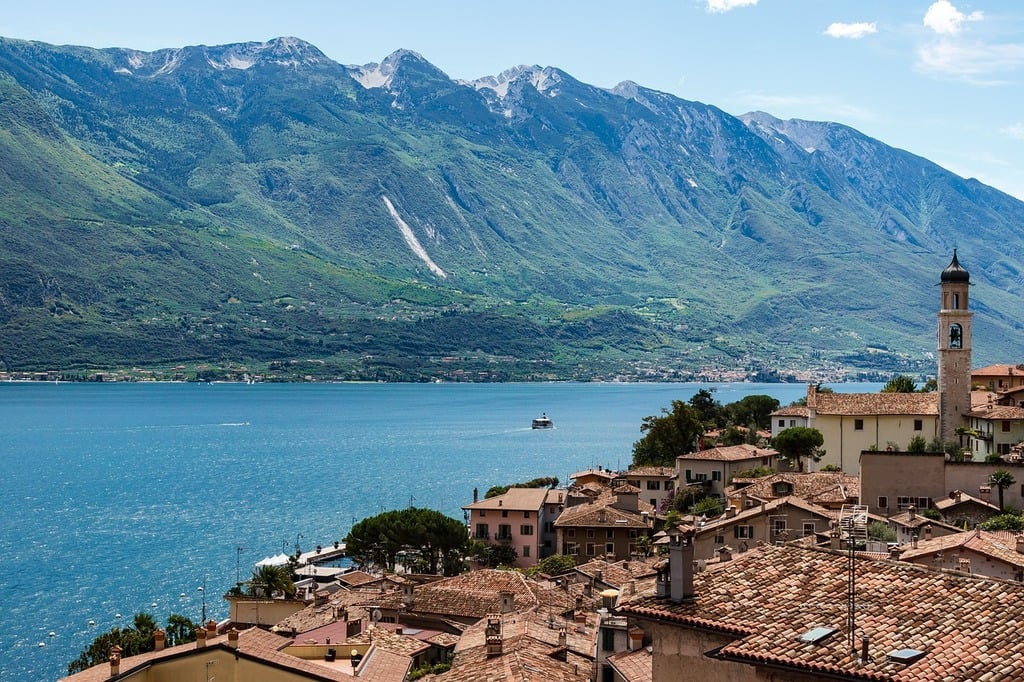
\includegraphics[width=\textwidth]{img/lake_garda_italy.jpg}
\tiny{Garda Lake, Italy (CC)}
          \column{0.58\textwidth}
          
Nice features : 
\begin{itemize}
  \item  almost close (within the watershed)
  \item  fish are mobile inside 
  \item  big enough mass of water  to buffer the climate changes
  \item  lot of human perturbations documented 
\end{itemize}

Two types of perturbations (\alert{controls}): 

\begin{itemize}
\item fish nutrients : human or industrial waste in the lake 
\item  fish harvesting 
\end{itemize}
\end{columns}
\end{footnotesize}
\vfill
How real interactions create patterns that differs from the theoretical ones ? 
 
\end{frame}

\begin{frame}{A lake story }



\alert{Paleolimnologists}  exist and are able to monitor a lake state over centuries.

\vfill

Example of a lake in Italy : 


\begin{footnotesize}
\begin{enumerate}
\item \alert{trophic equilibrium} $\approx$ no modification  for thousand years (2000 BC to 171 BC), even if surrounding change (steppes $\rightarrow$ grassland $\rightarrow$ forest)
\item Sudden \alert{shift} due to (external) perturbation  : Roman way (Via Cassia) in 171 BC, more people (waste). 
\item \alert{Eutrophication} : the environment becomes rich in nutrients N, P ($\implies$ subtle changes in hydrographic regimes : algae , plankton)  
\item \alert{New dynamics} and huge population changes (irreversible)
\end{enumerate}
\end{footnotesize}
\end{frame}





\begin{frame}{Common patterns}

\begin{footnotesize}
Same overall patterns in different countries (Italy, Canada, US) and fish species (sturgeon, herring, white fish ) 

\begin{itemize}
  \item prolonged high level of harvest 
  \item then  \alert{sudden drop} in populations(up to 4 order of magnitude in few years)
  \item appearance or disappearance of populations (flies, plancton, worms, fish)
  \item wide oscillations
  \item new domain of attraction establish 
\end{itemize}
\end{footnotesize}
\centering
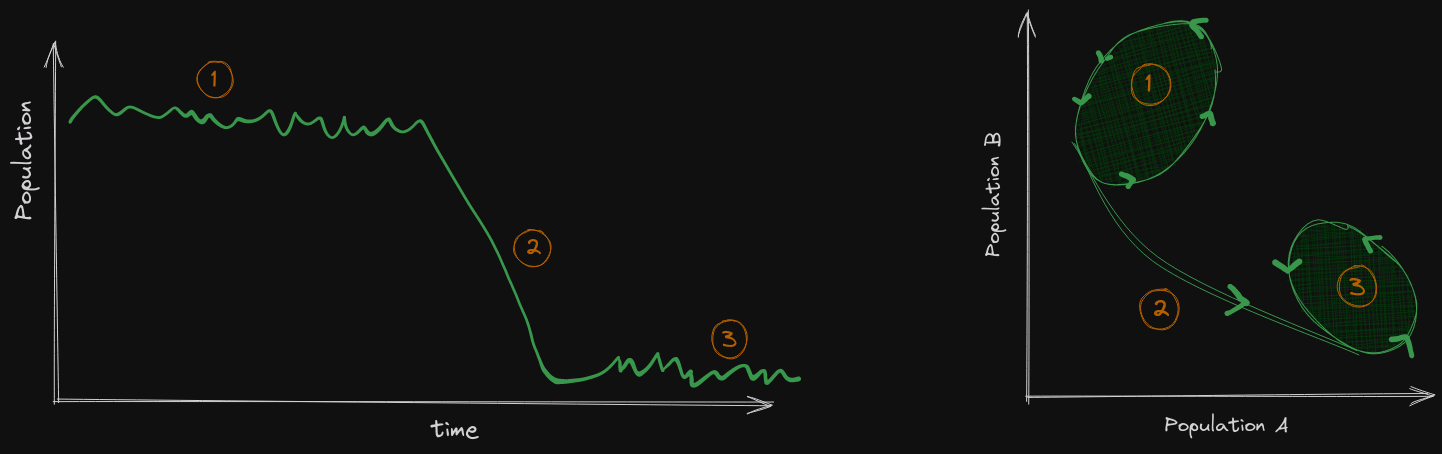
\includegraphics[height=0.4\textheight]{img/pattern_in_lake.png}


\end{frame}


\begin{frame}{Empirical Evidences}


\textit{"It is as is the population had been shifted by fishing pressure from a domain with a high equilibrium to one with a lower one"}

\vfill

\begin{footnotesize}
\begin{itemize}
  \item Fishing shifts the age structure of fish population towards younger ages (less opportunity to reproduce)
  \item Intense fishing pressure + changes in the chemicals of environment $\implies$ apparition of new predators , foreign competitors 
  \item Harvesting at the maximum of sustainable yield + a small mortality is \alert{sufficient} to cause the collapse
\end{itemize}


\end{footnotesize}




\end{frame}

\begin{frame}{Early Conclusions}

\begin{itemize}
\item Harvesting progressively reduced the \alert{resilience} of the fish population
\item Lakes have high but limited capacity to absorb perturbation
\item Once limits are crossed, the systems shifts to another domain
\item Distinct domain of attraction is not uncommon in closed systems 
\end{itemize}

\end{frame}


\begin{frame}{Vocabulary}


\begin{small}
\begin{block}{\alert{Driving variables}} $\approx$ "things that have an impact on others" \\
e.g. Land Cover, Rainfall, $t$ in $Pop_{fish}(t)$, Temperature, nutrient concentration, etc.
\end{block}
\vfill

\begin{block}{\alert{State variables}} $\approx$   observables , measures\\
 e.g. productivity of algae, Net ecosystem exchange of CO2, Fish population, etc.  
\end{block}
\vfill

\begin{block}{\alert{Resilience}}  "a measure of the \alert{persistence} of systems and of their \alert{ability to absorb change} and disturbance and still \alert{maintain
the same relationships} between populations or state variables"
\end{block}

\vfill
\end{small}

\tiny{Other disciplines have different meanings for driving and state variable}


\end{frame}





\begin{frame}{Extensions}



\begin{small}
\begin{itemize}
  \item Fecundity, mortality , competition and predation : \alert{Reproduction curves}
  \item  Environnement is not close nor random nor homogeneous : \alert{Spatial heterogeneity} 
  \end{itemize}


\end{small}
  
\end{frame}




\section{Reproduction curves}



\begin{frame}{Reproduction curves}
\begin{small}
Density of animals is "self regulated" : 

\begin{itemize}
  \item low density : difficulty to mate : density $\searrow$
  \item high density : competitions for mates, food, nesting sites  :  density $\searrow$
\end{itemize}

( also modifies neighbors in the trophic web)
\end{small}
\vfill 

Reproductions curves model that feedback 


\end{frame}


\begin{frame}{Reproduction curves}


\centering
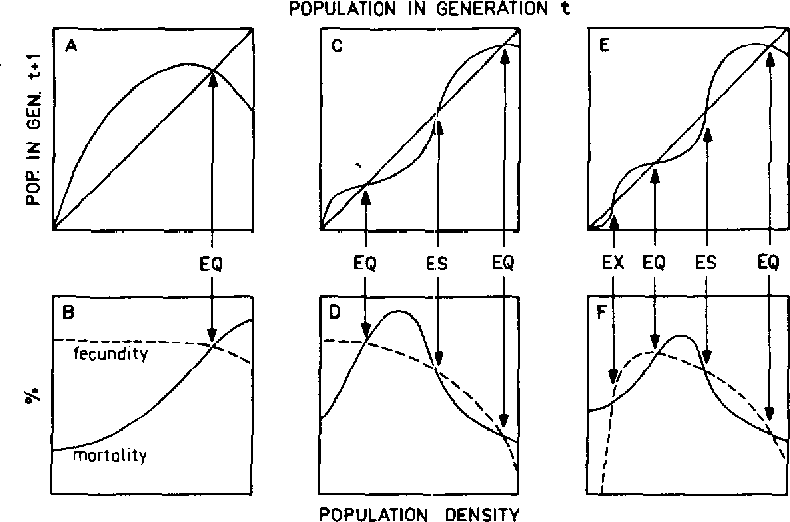
\includegraphics[height=0.5\textheight]{img/reproduction_curves.png}
\begin{footnotesize}
\begin{itemize}
\item EQ is \alert{equilibrium}
\item ES is \alert{escape threshold}
\item EX is \alert{extinction threshold}
\end{itemize}

  \end{footnotesize}

\end{frame}


\begin{frame}{Reproduction curves}

\vfill
\centering
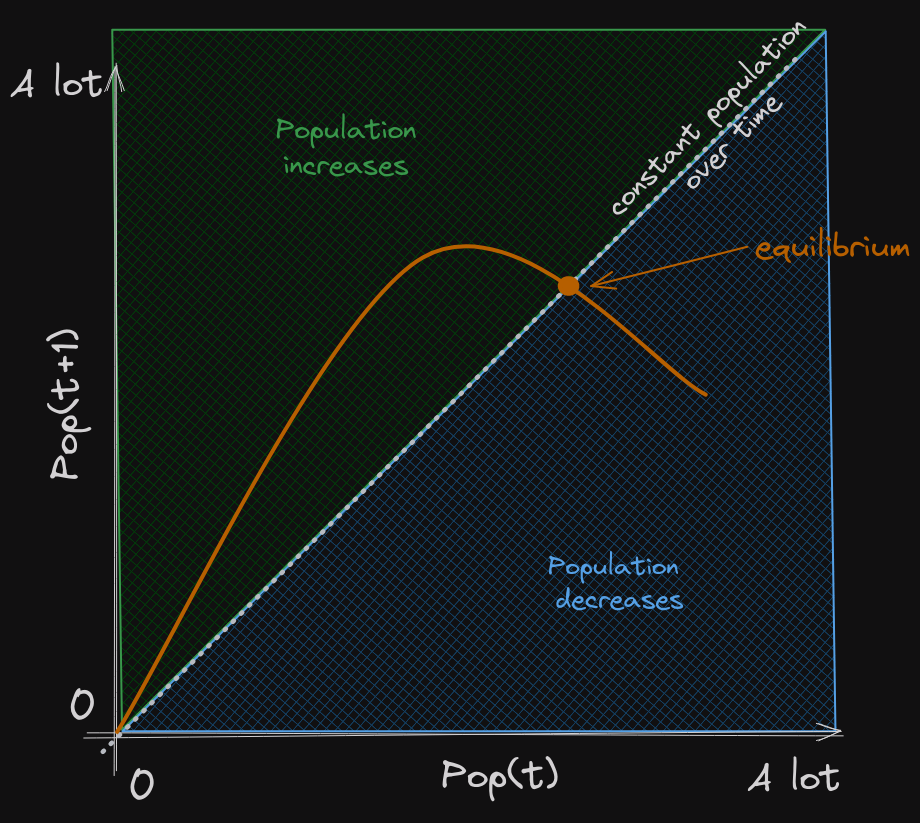
\includegraphics[height=0.8\textheight]{img/repro1.png}
\begin{footnotesize}
\end{footnotesize}

\end{frame}



\begin{frame}{Contributions of fecundity and mortality}

\vfill
\centering
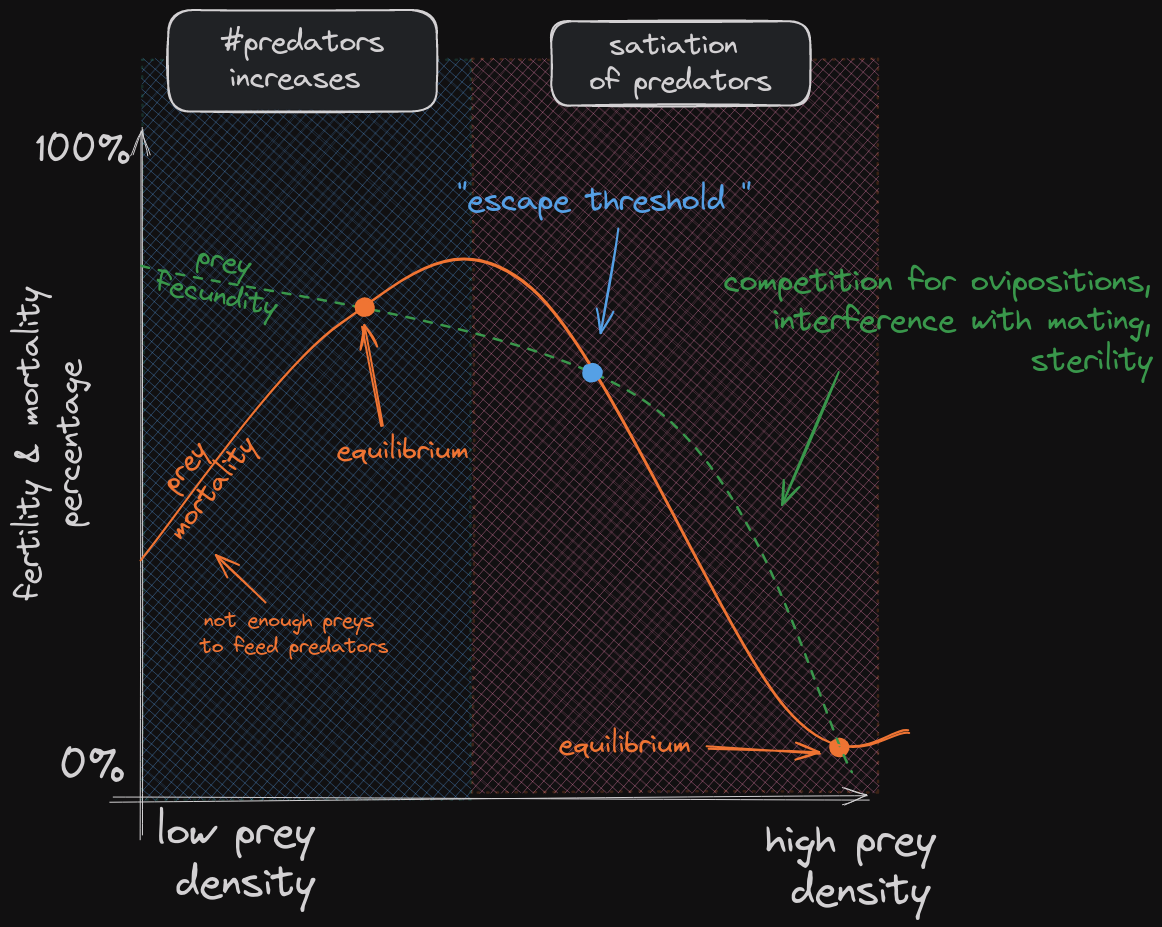
\includegraphics[height=0.8\textheight]{img/repro2.png}
\begin{footnotesize}
\end{footnotesize}

\end{frame}




\begin{frame}{Reproduction curves}


\centering
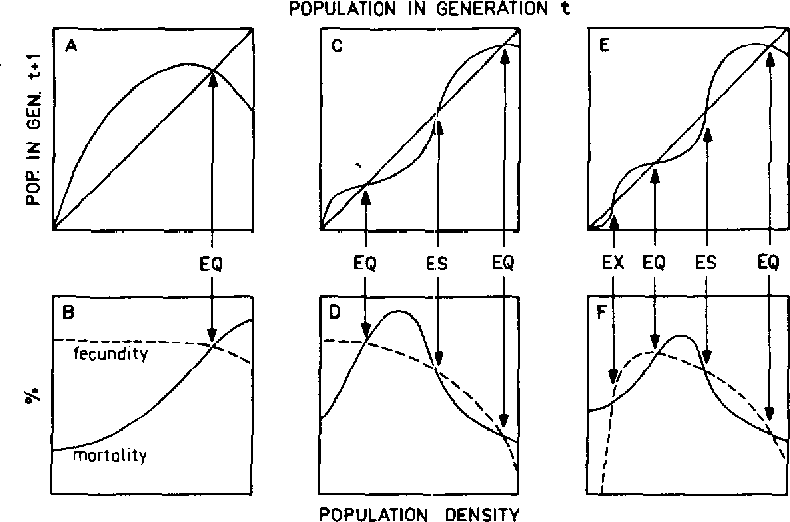
\includegraphics[height=0.5\textheight]{img/reproduction_curves.png}
\begin{footnotesize}
\begin{itemize}
\item B is not realistic, only show negative feedback of overcrowding
\item D is called \alert{Drosophilia -type} curve
\item F has been empirically demonstrated for \alert{insects}
\end{itemize}

  \end{footnotesize}

\end{frame}



\begin{frame}{Early Conclusions}


\centering
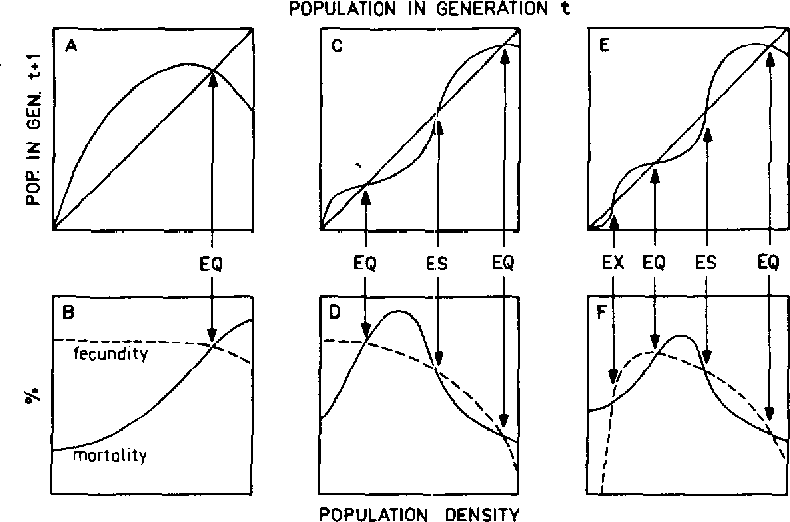
\includegraphics[height=0.5\textheight]{img/reproduction_curves.png}
\begin{footnotesize}
\begin{itemize}
\item C/D \& E/F are  found empirically  
\item Prey density threshold \alert{below which} prey become extinct
\item Prey density threshold \alert{above which} prey becomes extinct 
\item They are domains of attraction ! (no global stability)
\item more sinuosity is possible 
\end{itemize}

  \end{footnotesize}

\end{frame}






\section{Open real world systems}



\begin{frame}{Grass, trees and worms}


Longitudinal study of  spruce-fir-birch forest in Canada \\
\vfill
Infestation of \alert{budworms}, parasit of conifers.\\
\vfill
Budworm outbreaks appear after several dry years (7 outbreaks since 1700)
\vfill



\centering 
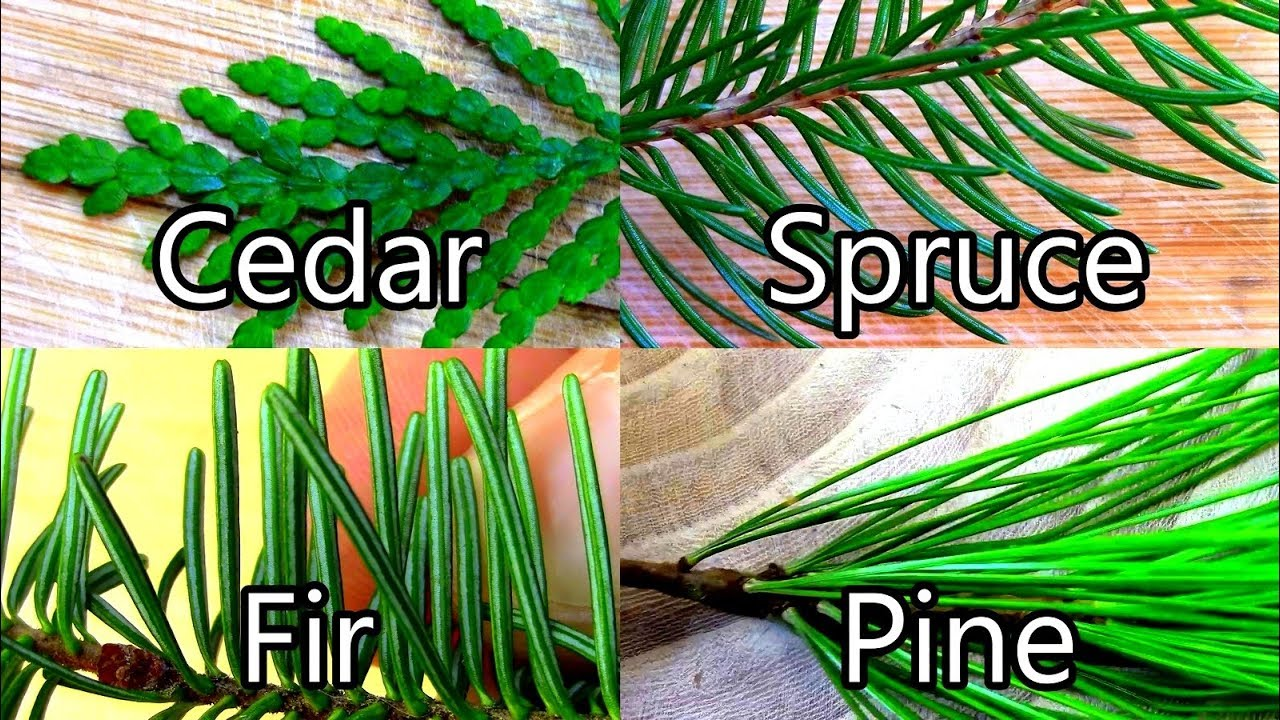
\includegraphics[height=0.3\textheight]{img/fir_spruce_pine_cedar.jpg}
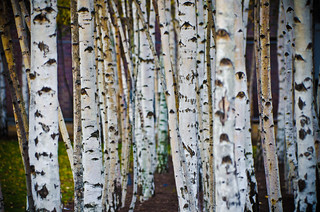
\includegraphics[height=0.3\textheight]{img/birch.jpg}
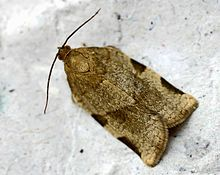
\includegraphics[height=0.3\textheight]{img/spruce_budworm.jpg}\\
\tiny{Choristoneura is a genus of moths in the family Tortricidae. Several species are serious pests of conifers, such as spruce}

\vfill

\end{frame}


\begin{frame}{Two regimes}


\begin{small}
\begin{columns}
\column{0.5\textwidth}
  \begin{block}{\alert{During outbreak}} 
  Worms population explodes ( $\times 10^4$) \\
  Firs collapse\\ 
  Spruce and birch survive (less prone to worms)
  \end{block}
\column{0.5\textwidth}
  \begin{block}{\alert{Between outbreaks}}
  Budworms regulated by parasites and predation\\
  Regeneration of fir $\rightarrow$ densification of trees\\
  Spruce and birch suffer from overcrowding, firs dominate 
  
  \end{block}
\end{columns}
\end{small}

\vfill

From trees perspective  :\\
 \alert{stable limit cycle}  with large amplitude

From budworms perspective : \\
  highly unstable system (population fluctuates widely)\\
 \alert{2 distinct basins} of attraction : one for standard population, one for outbreaks




\end{frame}
\begin{frame}{Species survival}


\begin{itemize} 
\item Spruce and birch would be excluded from the forest if no outbreak of budworms
\item Fir presist because of its regenerative powers and the interplay of forest growth rates and climatic conditions (that result in outbreak )
\item Fluctuations are essential to the maintaining of budworms : successive generations of trees assuring a continued food supply for future generations and persistence of the system $\{budworms, predators, trees\}$
\end{itemize}
\vfill
$\{Budworm, forest\}$ system is highly \alert{unstable} and yet highly \alert{resilient}
\vfill
Similar patterns with $\{salmon,predators\}$ and $\{grassland, trees, fires\}$  systems

\end{frame}





\section{Some pieces of Ecology  to remember / early conclusions}


\begin{frame}{Summary}



\alert{Stability} : the ability to return to an equilibrium after a disturbance\\
Stability characteristics  : degree of fluctuation  around the equilibrium states, returning to equilibrium time

\vfill

\alert{Resilience} : persistence of relations within the system, ability to absorb changes of state/driving  variables and still persist\\
The result of resilience is the persistence of a species, or a low probability of extinction 


\end{frame}



\begin{frame}{The Bowl}



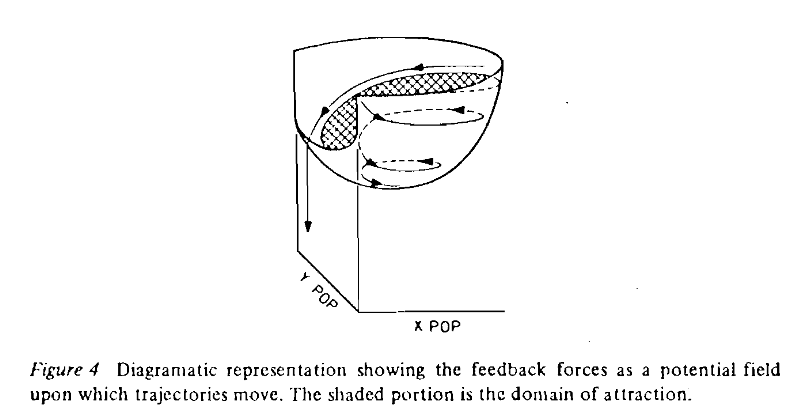
\includegraphics[height=0.8\textheight]{img/bowl.png}

\end{frame}




\begin{frame}{Summary}
\vfill
One can be resilient \alert{and} unstable ( cf. budworms)
\vfill

One can be stable but not resilient :  population in almost constant climatic  conditions for a long period can lose the ability to adapt to disturbance (cf . fish in lake) 

\vfill
When systems are \alert{open}, and the species able to \alert{disperse}, they tend to be resilient  (e.g. pests like locusts)

\vfill

\end{frame}
\begin{frame}{Complex systems vulgate}


 Common knowledge is that diversity is linked with stability. \\

 Stability is roughly the number of links in a trophic web 

\vfill

 
 Complex systems tend to fluctuate more than simple ones.

\vfill

 More species $\implies$ more domains of attraction. \\

 Despite higher fluctuation, overall persistence might be increased. 
 



\end{frame}


\section{Final words}

\begin{frame}{Take home messages}

\begin{itemize}
 \item Nature is scary (for modelers)
 \item Everything, everywhere, all at once  (has an impact in the ecosystem dynamics)
 \item Completely quantifying interactions and states  is impossible 
 \item Traditional/analytical tools are seldom useful (simulation can help)
 \item Equilibrium view is not that useful, nor true
 \item Several basins of attraction, limit cycles, random perturbations.
\end{itemize}

\end{frame}


\begin{frame}{Resilience in other disciplines}

\begin{small}
\alert{Engineering resilience} :   the ability of a system to return to an equilibrium state after a temporary perturbation by measuring how quickly a system’s equilibrium is restored (Pimm 1984, Holling 1996).

\vfill

\alert{Socio-technical resilience}  i.e. common points in a lot of resilience definitions : 
\begin{itemize}
  \item  \alert{Adaptability} and flexibility 
  \item  The ability to \alert{self-organize}
  \item  The ability to build and increase the capacity for \alert{learning and adaptation}
  \item  The ability to maintain \alert{links}  with other sytems 
  \end{itemize}
\end{small}


\end{frame}



\begin{frame}{My POV, chapter I}

\begin{itemize}
\item  domain of attractions are like the algebra they come from  : conceptual/imaginary elements and operations 
\item  Sometimes a tiny fraction of the real world can be modelled by combining these elements
\item  remind me of thermodynamics : 
\begin{itemize}
  \item  only states can be modeled,  
  \item  $\implies$ only $\Delta$s can be computed
  \item  how real transitions occur is untractable/mystery 
  \end{itemize}
\item  Holling's original and iconoclast vision : \alert{\textit{There is (almost) no (static) equilibrium in Nature}}
\end{itemize}


\end{frame}



\begin{frame}{My POV, chapter II}
\begin{itemize}
\item one of the best paper I ever read
\item talented writing  esp. progressive complexification 
\item seems to be a must read in the field ( similar to Dawkins' Selfish gene paper)
\vfill
\item major impact in a lot of disciplines : resilience is now a buzzword
\item easy to learn, hard to master  concepts
\item Holling proposes a \textit{paradigm} :  can be applied to almost everything
\end{itemize}

\end{frame}


\begin{frame}{Confusing Resilience with  Robustness : Never Again}

\centering
 Which one is the most resilient ? 


\includegraphics[height=0.8\textheight]{img/wolverine_colossus.jpg}

\tiny{Cover by Mark Bagley,  © Marvel }

\end{frame}







\begin{frame}{References}


The paper : \url{https://pure.iiasa.ac.at/id/eprint/26/1/RP-73-003.pdf}

Ecosystem models wikipedia page (a good introduction) : \url{https://en.wikipedia.org/wiki/Ecosystem_model} \\

Holling's carreer overview \url{ https://www.nature.com/articles/s41893-019-0425-9\#ref-CR4}

Netlogo Cinematic Universe : \url{https://ccl.northwestern.edu/netlogo/}


\end{frame}




\begin{frame}[standout]

\centering
Thank You\\
\vfill
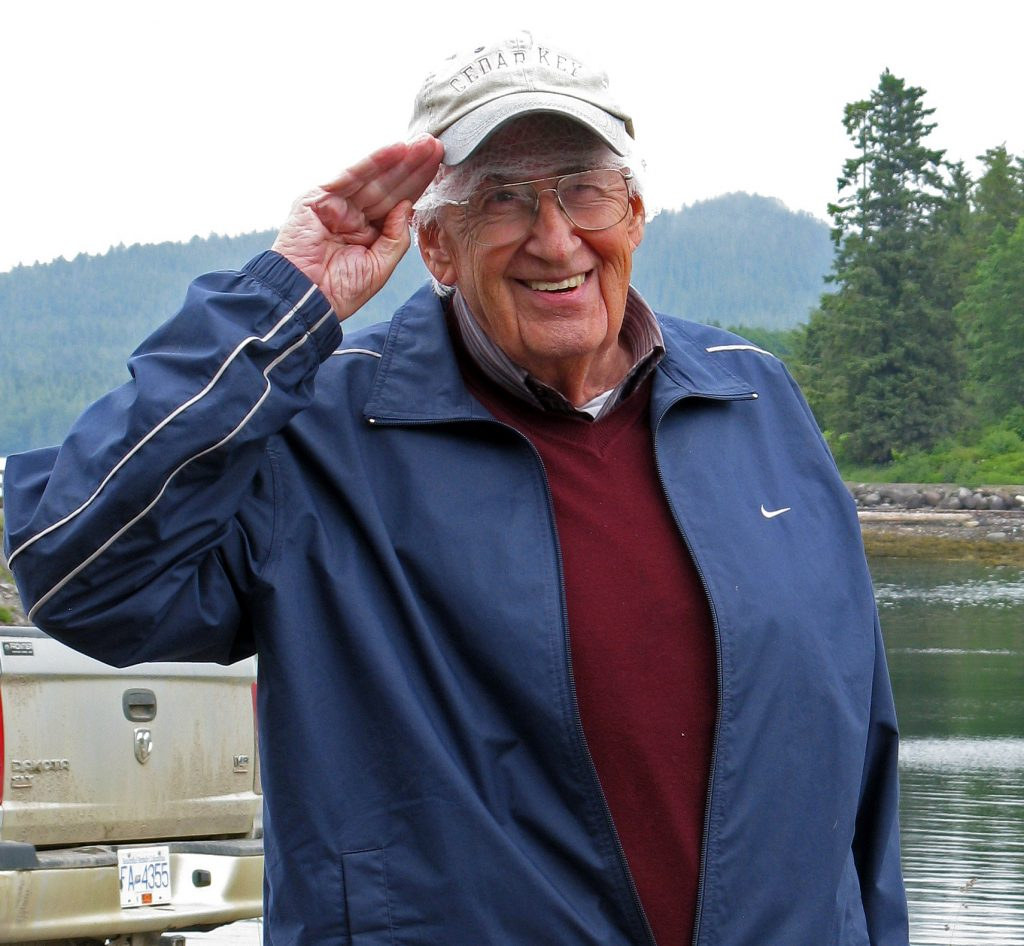
\includegraphics[height=0.9\textheight]{img/holling2.jpg} \\
\tiny{photo from Ecotrust Canada website}
  
\end{frame}






\begin{comment}


\section{Predator and prey}



@article{Pethybridge2018ImprovingME,
  title={Improving Marine Ecosystem Models with Biochemical Tracers.},
  author={Heidi R. Pethybridge and C. Anela Choy and Jeffrey Joseph Polovina and Elizabeth A. Fulton},
  journal={Annual review of marine science},
  year={2018},
  volume={10},
  pages={
          199-228
        },
  url={https://api.semanticscholar.org/CorpusID:207741887}
}
\end{comment}

\end{document}
